\section{Methodik}
\label{sec:methodik}

Die Analyse gliedert sich in drei aufeinander aufbauende Schritte: Datenerhebung und Qualitätsprüfung, Sentiment-Analyse sowie Korrelationsmodellierung. Jeder Schritt entspricht einem Jupyter-Notebook (\texttt{01\_data\_quality\_eda.ipynb}, \texttt{02\_sentiment\_analysis.ipynb}, \texttt{03\_correlation\_modeling.ipynb}).

% ─────────────────────────────────────────────────────────────────────────────
\subsection{Datenerhebung und explorative Qualitätsprüfung}
\label{subsec:eda}

\subsubsection*{Vorgehen}

Im ersten Schritt wurde die strukturelle Qualität der erhobenen Daten geprüft.
Grundlage bildeten die in einer SQLite-Datenbank gespeicherten Tweets, Tweet-Snapshots und Intraday-Preissnapshots sowie separat vorliegende historische Tagespreise, die über die Bibliothek \textit{yfinance} bezogen und in einer CSV-Datei abgelegt wurden. Ziel dieses Schritts war es, Datenlücken, Abdeckungsunterschiede zwischen Unternehmen und potenzielle Verzerrungen sichtbar zu machen, bevor inhaltliche Sentiment-Scores berechnet wurden. Dazu wurden Zeitstempel vereinheitlicht, ein Startzeitraum ab dem 01.\,01.\,2026 angewendet und die Analyse auf die in einer Konfigurationsdatei definierten Fokus-Ticker beschränkt.

Für die inhaltliche Zuordnung der Tweets zu den Fokus-Unternehmen wurde ein zweistufiges Matching-Verfahren verwendet. Im ersten Schritt wurden vorhandene Cashtags bzw. Symbolspalten direkt bekannten Ticker-Aliasen zugeordnet. Im zweiten Schritt wurden Tweets ohne Symbolangabe anhand regulärer Ausdrücke auf Unternehmensnamen, Cashtags und markenspezifische Begriffe geprüft. Dadurch konnten auch Beiträge erfasst werden, die nicht explizit mit einem Börsenkürzel versehen waren. Ergänzend wurden Tweets mit und ohne substanziellen Inhalt unterschieden: URLs, Mentions und Cashtags wurden entfernt und nur Beiträge mit mindestens 20~verbleibenden Zeichen als inhaltlich aussagekräftig markiert.

Ein weiterer methodischer Bestandteil war die Identifikation strukturell auffälliger Tweets. Dazu wurden Retweets über das Präfix \enquote{RT @} markiert sowie Kandidaten für nicht-organische Aktivität geprüft. Engagement-Snapshots wurden zusammengeführt, um erste Aussagen über Reichweite und Interaktionsdynamik zu ermöglichen. Viral aktive Tweets wurden über das 95.\,Perzentil der Engagement-Velocity (Likes pro Minute zwischen erstem und letztem Snapshot) identifiziert.

\subsubsection*{Datensätze}

Verwendet wurden die Tabellen \texttt{tweets}, \texttt{tweet\_snapshots} und \texttt{price\_snapshots} aus der SQLite-Datenbank sowie die historischen Tagespreise aus \texttt{prices.csv}. Die Tweets enthalten Autor, Inhalt, Posting-Zeitpunkt und teils ein extrahiertes Symbol. Die Snapshots liefern Engagement-Metriken (Likes, Retweets) und kursbezogene Momentaufnahmen.

\subsubsection*{Beobachtungen}

Die Analyse ergab, dass die Ticker-Zuweisung initial für mehrere Unternehmen zu geringe Abdeckungen lieferte. Als Ursache wurden zu eng gefasste Wortgrenzen in den regulären Ausdrücken identifiziert: Ausdrücke der Form \texttt{\textbackslash bWORD\textbackslash b} konnten zusammengesetzte Hashtags wie \textit{\#TeslaStock} oder \textit{\#NIBEHeatPump} nicht erfassen, da der Wortgrenzenoperator einen Folgebuchstaben nicht zulässt. Die Muster wurden daraufhin angepasst. Tabelle~\ref{tab:coverage} zeigt die resultierende Abdeckung je Ticker.

\begin{table}[H]
\centering
\caption{Abdeckung der Fokus-Ticker im bereinigten Datensatz (Zeitraum ab 01.01.2026)}
\label{tab:coverage}
\begin{tabular}{lrr}
\toprule
\textbf{Ticker} & \textbf{Tweet-Tage} & \textbf{Sentiment-Tage} \\
\midrule
TSLA   & 124 & 68 \\
VWAGY  &  91 & 53 \\
XOM    &  72 & 41 \\
BYDDY  &  59 & 34 \\
BP     &  50 & 27 \\
TTE    &  38 & 23 \\
6503.T &  29 & 17 \\
6367.T &  17 & 11 \\
E      &   9 &  7 \\
SHEL   &   8 &  5 \\
CARR   &   9 &  3 \\
NIBE-B.ST &  2 &  1 \\
\bottomrule
\end{tabular}
\end{table}

% ─────────────────────────────────────────────────────────────────────────────
\subsection{Sentiment-Analyse}
\label{subsec:sentiment}

\subsubsection*{Modellauswahl}

Für die Sentiment-Klassifikation wurde \texttt{cardiffnlp/twitter-xlm-roberta-base-sentiment} als Primärmodell eingesetzt \autocite{loureiro2022timelms}. Die Wahl dieses Modells war methodisch sinnvoll, weil der Datensatz nicht nur englische, sondern auch deutsch-, französisch- und japanischsprachige Tweets enthält. Das Modell basiert auf XLM-RoBERTa \autocite{conneau2020unsupervised} und ist speziell auf Twitter-Daten trainiert. Es klassifiziert jeden Eingabetext in eine von drei Klassen: \textit{Positive}, \textit{Neutral}, \textit{Negative}. Zusätzlich stellt es Klassenwahrscheinlichkeiten bereit, aus denen ein kontinuierlicher Compound-Score gebildet wurde:

\begin{equation}
\text{xlm\_compound} = P(\text{positive}) - P(\text{negative}) \in [-1,\, 1]
\label{eq:compound}
\end{equation}

Als Baseline wurde ergänzend VADER (Valence Aware Dictionary and sEntiment Reasoner) eingesetzt \autocite{hutto2014vader}. Da VADER auf einem englischen Lexikon basiert, ist es für nicht-englische Tweets nicht valide. Es diente daher ausschließlich als Vergleichsmaßstab für den englischsprachigen Anteil des Datensatzes.

\subsubsection*{Datenfilterung}

Vor der Modellinferenz wurden zwei Filtermaßnahmen angewendet:

\begin{enumerate}[noitemsep]
\item \textbf{Bot-Filterung:} Als Bot-Kandidat wurde jeder Account definiert, der keine Follower besitzt und zugleich mindestens drei Tweets im Datensatz veröffentlicht hat. Diese Regel ist als konservativer Proxy für nicht-organische Aktivität zu verstehen.
\item \textbf{Content-Filter:} Die Inferenz wurde ausschließlich auf Tweets angewendet, die nach Entfernung von URLs, Mentions und Cashtags noch mindestens 20~Zeichen enthielten.
\end{enumerate}

Die Sprache jedes Tweets wurde außerdem mit \textit{langdetect} automatisch erkannt, um die Übereinstimmung zwischen XLM-RoBERTa- und VADER-Ergebnissen sprachspezifisch auswerten zu können.

\subsubsection*{Retweet-Separation}

Original-Tweets und Retweets wurden getrennt verarbeitet, um zu vermeiden, dass die bloße Weiterverbreitung von Inhalten das Sentiment-Signal verzerrt. Als Retweet wurde jeder Beitrag eingestuft, der mit dem Präfix \enquote{RT @} beginnt. Im vorliegenden Datensatz enthielten alle gecrawlten Tweets originären Inhalt; die Trennung war daher analytisch irrelevant, methodisch aber korrekt implementiert.

\subsubsection*{Tägliche Aggregation}

Auf Tweet-Ebene erzeugte Sentiment-Scores wurden je Fokus-Ticker und Kalendertag aggregiert. Die täglichen Aggregate umfassen:

\begin{itemize}[noitemsep]
\item \texttt{mean\_xlm\_compound}: ungewichteter Mittelwert des Compound-Scores
\item \texttt{pct\_positive}, \texttt{pct\_negative}: Anteile positiver und negativer Tweets
\item \texttt{mean\_vader\_en}: mittlerer VADER-Score (nur englische Tweets)
\item \texttt{weighted\_xlm\_compound}: follower-gewichteter Compound-Score als Reichweiten-Proxy
\end{itemize}

Der follower-gewichtete Score gewichtet den Compound-Wert jedes Tweets proportional zu den Follower-Zahlen des Autors:

\begin{equation}
\text{weighted\_xlm} = \frac{\sum_{i} f_i \cdot c_i}{\sum_{i} f_i}
\label{eq:weighted_compound}
\end{equation}

wobei $f_i$ die Follower-Zahl und $c_i$ den Compound-Score von Tweet $i$ bezeichnen. Dieses Signal dient als primäres Sentiment-Maß in der Korrelationsanalyse, da es die Reichweite einzelner Beiträge berücksichtigt.

Abbildung~\ref{fig:follower_weighting} zeigt den Vergleich von ungewichtetem und follower-gewichtetem Compound-Score je Ticker. Die meisten Ticker liegen nahe der Diagonalen, was auf geringe Gewichtungseffekte hindeutet.

\begin{figure}[H]
  \centering
  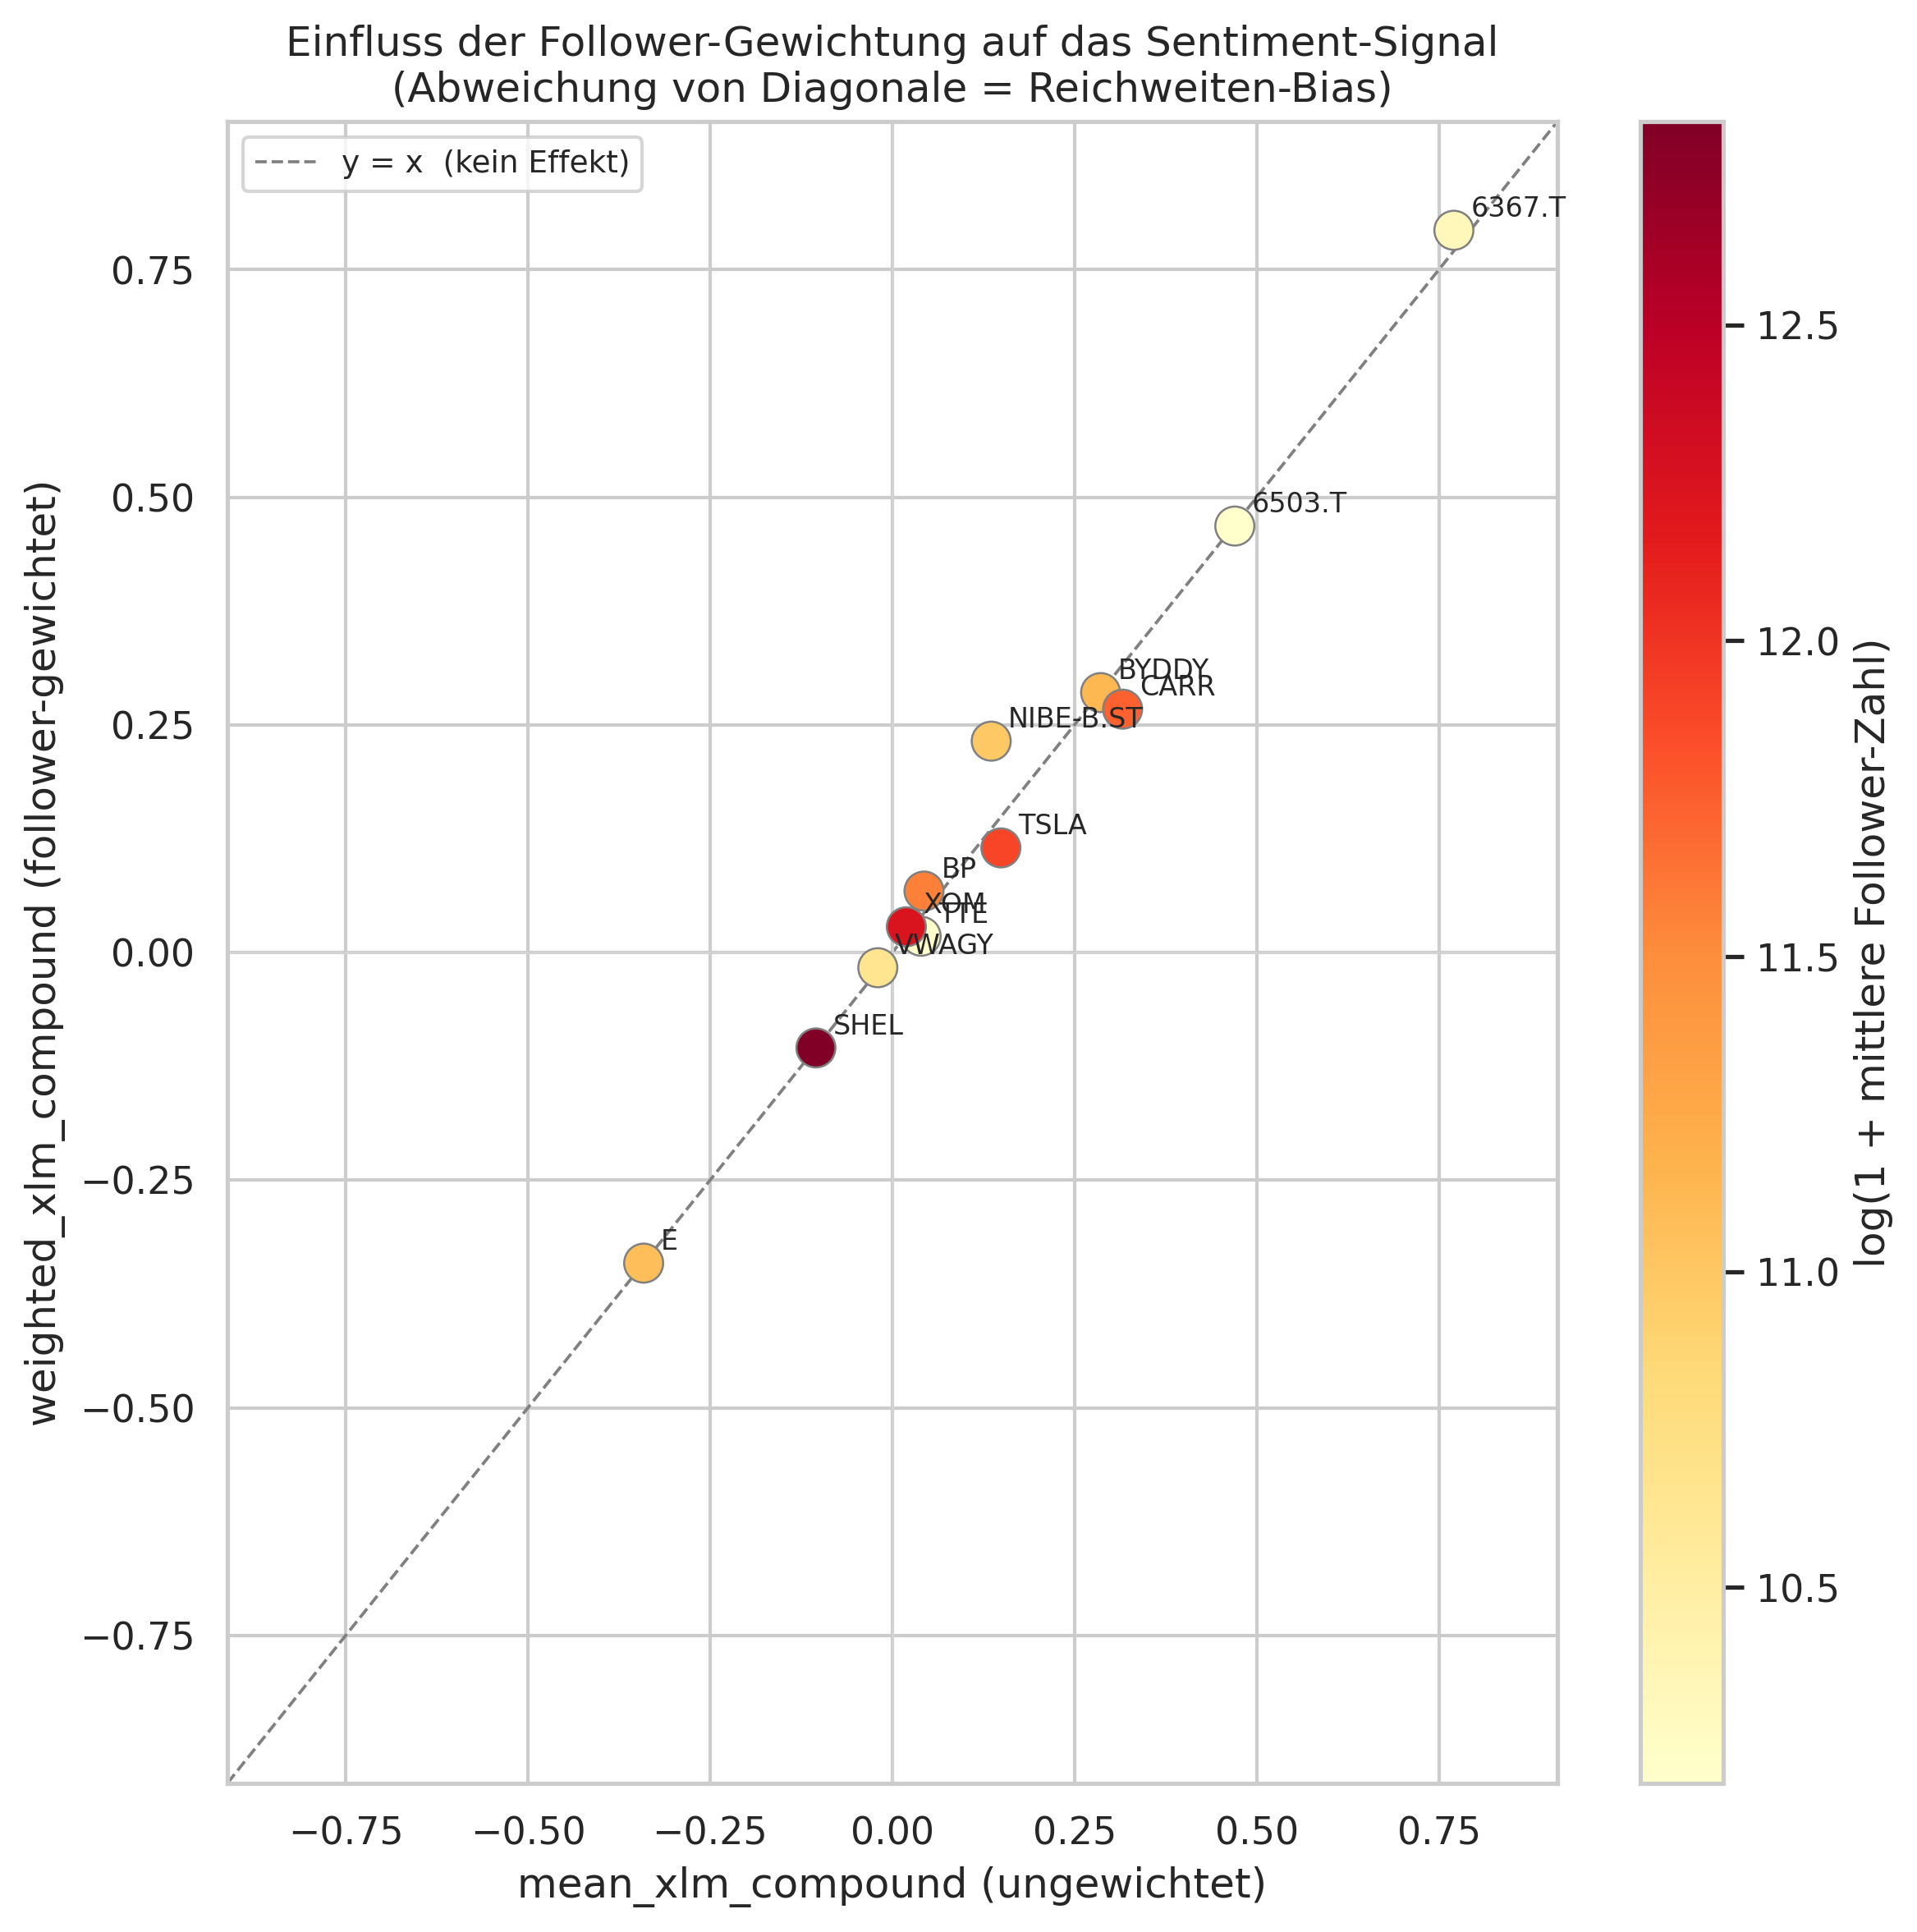
\includegraphics[width=0.72\textwidth]{figures/02_sentiment_analysis/04_follower_weighting_scatter.png}
  \caption{Ungewichteter vs.\ follower-gewichteter mittlerer Compound-Score je Fokus-Ticker. Punkte auf der Diagonalen zeigen keinen Reichweiten-Bias; Einfärbung nach $\log(1 + \text{mittlere Follower-Zahl})$.}
  \label{fig:follower_weighting}
\end{figure}

\subsubsection*{Datensätze}

Als Input dienten die Tweets aus der SQLite-Datenbank. Als Output wurden folgende Parquet-Dateien erzeugt:

\begin{itemize}[noitemsep]
\item \texttt{tweets\_with\_sentiment\_original.parquet} (2\,266 Zeilen, tweet-level)
\item \texttt{daily\_sentiment\_original.parquet} (508 Zeilen, Primärinput für NB03)
\end{itemize}

% ─────────────────────────────────────────────────────────────────────────────
\subsection{Korrelationsmodellierung}
\label{subsec:korrelation}

\subsubsection*{Daten und Zusammenführung}

Als Primärinput für die Korrelationsanalyse wurde \texttt{daily\_sentiment\_original.parquet} verwendet. Retweets wurden bewusst aus der Hauptanalyse ausgeschlossen. Als zentrales Sentiment-Signal diente der follower-gewichtete Compound-Score \texttt{weighted\_xlm\_compound} gemäß Gleichung~\eqref{eq:weighted_compound}.

Die Tagesrendite wurde aus historischen Tagespreisen über einfache prozentuale Veränderung des adjustierten Schlusskurses berechnet:

\begin{equation}
r_t = \frac{P_t - P_{t-1}}{P_{t-1}}
\label{eq:return}
\end{equation}

Die Zusammenführung erfolgte über einen Inner-Join auf Ticker und Datum, sodass nur Tage mit sowohl validem Sentiment-Score als auch gültigem Renditewert in die Analyse eingingen.

\subsubsection*{Overlap-Report und Methoden-Eligibility}

Statt einer globalen Mindeststichprobenschwelle, die Ticker still ausschließt, wurde ein Overlap-Report erstellt. Dieser dokumentiert für jeden Fokus-Ticker die Anzahl der Sentiment-Tage, Preis-Tage und tatsächlich überlappenden Tage sowie methodenspezifische Eligibility-Flags:

\begin{itemize}[noitemsep]
\item \textbf{Pearson/Spearman:} mindestens 5 gepaarte Beobachtungen pro Lag
\item \textbf{Rolling-Korrelation:} mindestens 30 Überlappungstage
\item \textbf{Granger-Test:} mindestens 30 Beobachtungen
\item \textbf{Event-Study:} mindestens 20 Basistage und mindestens 5 Ereignisse je Richtung
\end{itemize}

Dieses Vorgehen stellt sicher, dass alle Ticker im Analysebericht sichtbar bleiben, während gleichzeitig statistisch zu dünne Teilanalysen transparent als nicht belastbar gekennzeichnet werden.

\subsubsection*{Methode 1: Lag-Korrelation (Pearson und Spearman)}

Für Lags $l \in \{0, 1, 2, 3\}$ wurde berechnet, ob der Sentiment-Score am Tag $t$ mit der Rendite am Tag $t+l$ korreliert. Lag~0 entspricht einem gleichzeitigen Zusammenhang, Lags~1--3 einem potenziellen Vorlauf des Sentiments gegenüber der Rendite:

\begin{equation}
r_{\text{Pearson}}(l) = \text{corr}\!\left(\text{sentiment}_t,\; r_{t+l}\right)
\label{eq:pearson_lag}
\end{equation}

Neben dem linearen Pearson-Koeffizienten wurde auch der rangbasierte Spearman-Koeffizient berechnet, um Robustheit gegenüber Ausreißern zu prüfen.

Da für bis zu zehn Ticker bei je vier Lags potenziell 40 Tests durchgeführt werden, wurden alle $p$-Werte mit der Benjamini-Hochberg-Methode (False Discovery Rate, FDR) korrigiert \autocite{benjamini1995controlling}. Berichtete Signifikanz bezieht sich stets auf den adjustierten Wert $p_{\mathrm{adj}}$. Ergänzend wurden 95\,\%-Konfidenzintervalle für den Pearson-Koeffizienten über die Fisher-z-Transformation berechnet:

\begin{equation}
z = \operatorname{arctanh}(r), \quad
\mathrm{SE}_z = \frac{1}{\sqrt{n-3}}, \quad
\mathrm{KI}_{95\%} = \bigl[\tanh(z - 1{,}96 \cdot \mathrm{SE}_z),\; \tanh(z + 1{,}96 \cdot \mathrm{SE}_z)\bigr]
\label{eq:fisher_ci}
\end{equation}

\subsubsection*{Methode 2: Rolling-Korrelation}

Für Ticker mit mindestens 30 überlappenden Tagen wurde ein gleitender Pearson-Korrelationskoeffizient mit einem Fenster von 30 Handelstagen berechnet. Dieser dient dazu, zeitliche Instabilität oder Phasenwechsel im Zusammenhang sichtbar zu machen, die bei aggregierten Gesamtmaßzahlen verborgen bleiben würden.

\subsubsection*{Methode 3: Granger-Kausalitätstest}

Der Granger-Test \autocite{granger1969investigating} prüft, ob vergangenes Sentiment einen zusätzlichen Beitrag zur Vorhersage zukünftiger Renditen leistet -- über die Autokorrelation der Renditen hinaus. Technisch wird ein VAR(l)-Modell geschätzt und über einen F-Test getestet, ob die Sentiment-Lags in der Renditegleichung statistisch signifikant sind. Zur Überprüfung der Stationaritätsvoraussetzung wurden die Sentiment- und Renditereihen jedes für den Granger-Test in Frage kommenden Tickers vorab mit dem Augmented-Dickey-Fuller-Test (ADF) auf Einheitswurzeln geprüft \autocite{dickey1979distribution}. Getestet wurden Lags 1 bis 3. Zu beachten ist, dass Granger-Kausalität keine echte Kausalität im wissenschaftlichen Sinne belegt, sondern lediglich Vorhersageverbesserung anzeigt \autocite{granger1969investigating}.

\subsubsection*{Methode 4: Event-Study}

In der Event-Study wurden Tage identifiziert, an denen der Sentiment-Score um mehr als eine Standardabweichung vom Ticker-Mittelwert abwich:

\begin{equation}
\text{Ereignis}^+ : \; s_t > \bar{s} + \sigma_s, \qquad
\text{Ereignis}^- : \; s_t < \bar{s} - \sigma_s
\label{eq:event_condition}
\end{equation}

Als abnormale Rendite wurde die Differenz zwischen der tatsächlichen Rendite und der Tagesrendite des S\&P\,500-Index (\texttt{\textasciicircum GSPC}) als externem Marktbenchmark definiert. Die S\&P\,500-Daten wurden über \textit{yfinance} bezogen. Diese Wahl vermeidet den methodischen Fehler, den Benchmark aus den Focus-Tickern selbst zu berechnen, was zu einem zirkulären Vergleich geführt hätte. Über alle Ereignisse wurde ein Durchschnitts-CAR-Profil (Cumulated Abnormal Return) im Fenster $t \in [-5, +5]$ Handelstagen berechnet.
